\newcommand{\tableResource}{
		\begin{center}
		\begin{tabular}{|p{3.5cm}|c|c|c|c|c|c|c|}
			\hline
			\textbf{Nominativi} &
			\textbf{Ad} &
			\textbf{Re} &
			\textbf{An} &
			\textbf{Ve} &
			\textbf{Pj} &
			\textbf{Pr} &
			\textbf{Totali}\\
			\hline
		}
\newcommand{\tableResourceTwo}{
		\begin{center}
		\begin{tabular}{|p{4cm}|c|c|c|c|c|c|c|}
			\hline
			\textbf{Nominativi} &
			\textbf{Ad} &
			\textbf{Re} &
			\textbf{An} &
			\textbf{Ve} &
			\textbf{Pj} &
			\textbf{Pr} &
			\textbf{Ore Totali} &
			\textbf{Ore Rendicontate}\\
			\hline
		}
\newcommand{\tableEco}{
		\begin{center}
		\begin{tabular}{|l|c|r|}
			\hline
			\textbf{Ruolo} &
			\textbf{Ore} &
			\textbf{Costo}\\
			\hline
}
\section{Suddivisione del lavoro e proposta economica}
\label{lavoroEconomico}
\subsection{Premessa}
I componenti del gruppo \authorName{} dovranno rivestire almeno una volta i ruoli identificati nella sezione \ref{defRuoli}.Vediamo ora in dettaglio la suddivisione dei ruoli per le risorse a disposizione per ogni fase. Verranno inoltre presentati in questa sezione i prospetti economici delle ore preventivate per i ruoli, in ciascuna fase individuata precedentemente nella sezione \ref{Pianificazione}.
Occorre ricordare che le attività della fase \textbf{A (FA)} non sono imputabili al proponente, di conseguenza le ore impiegate in questa fase non sono calcolate nelle ore rendicontate per il calcolo della retribuzione, ma verranno comunque proposte per dare un'immagine di insieme. Riportiamo nuovamente in questa sezione, le ore a ruoli viste nella sezione \ref{CalendarioAttività} in modo tale da avere disponibili, sia le ore divise tra i ruoli, sia il costo del ruolo nella fase in esame. Inoltre per il calcolo dei costi ci riferiamo alla tabella contenuta nella pagina \url{http://www.math.unipd.it/~tullio/IS-1/2013/Progetto/PD01b.html} nella sezione \emph{Offerta tecnico-economica}.
\pagebreak
%%%%%%%%%%%%%%%%%%%%%%%%%%%%%%%%%%%%%%%%%%%%%%%%%%
% ANALISI
%%%%%%%%%%%%%%%%%%%%%%%%%%%%%%%%%%%%%%%%%%%%%%%%%%
\subsection{Fase A}
\label{AnalisiLav}
\subsubsection{Suddivisione del lavoro}
\label{lavoroA}
Nella FA, ciascun componente dovrà rivestire i ruoli come illustrato nella tabella seguente:
\begin{table} [!h]
\tableResource
Adami Alberto & 10 & & 7 & 3 & & & 20\\
Bissacco Nicolò & 10 & 4 & 7 & & & & 21\\
Feltre Beatrice & & 8 & 12 & & & & 20\\
Luisetto Luca & & & 13 & 8 & & & 21\\
Magnabosco Nicola & & 6 & & 15 & & & 21\\
Martignago Jimmy & & & 15 & 6 & & & 21\\
Scapin Davide & & & 11 & 9 & & & 20\\ \hline
\end{tabular}\caption{Ore a Componente per Ruolo, Fase A} \end{center}
\end{table}

I valori sono riassunti nel seguente grafico che visualizza le ore che un membro ha ricoperto in un determinato ruolo.
\begin{figure}[h!]
	\centering
	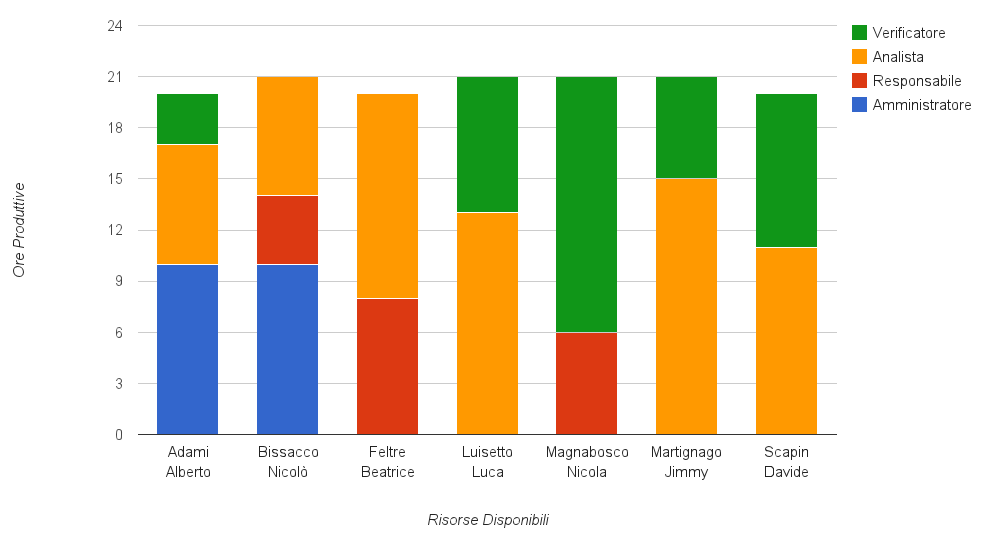
\includegraphics[width=1.2\linewidth]{./content/Immagini/prospetti/risorseAn.png}
	\caption{Ore per Componente, Fase A}
\end{figure}

Il diagramma che segue rappresenta le attività effettive assegnate ad ogni risorsa e la percentuale di tempo dedicato ad essa, evidenziando in rosso, quelle risorse che si trovano sovraccaricate e in verde quelle invece che sono sottoccupate.
\begin{landscape}
\begin{figure}[h]
	\centering
	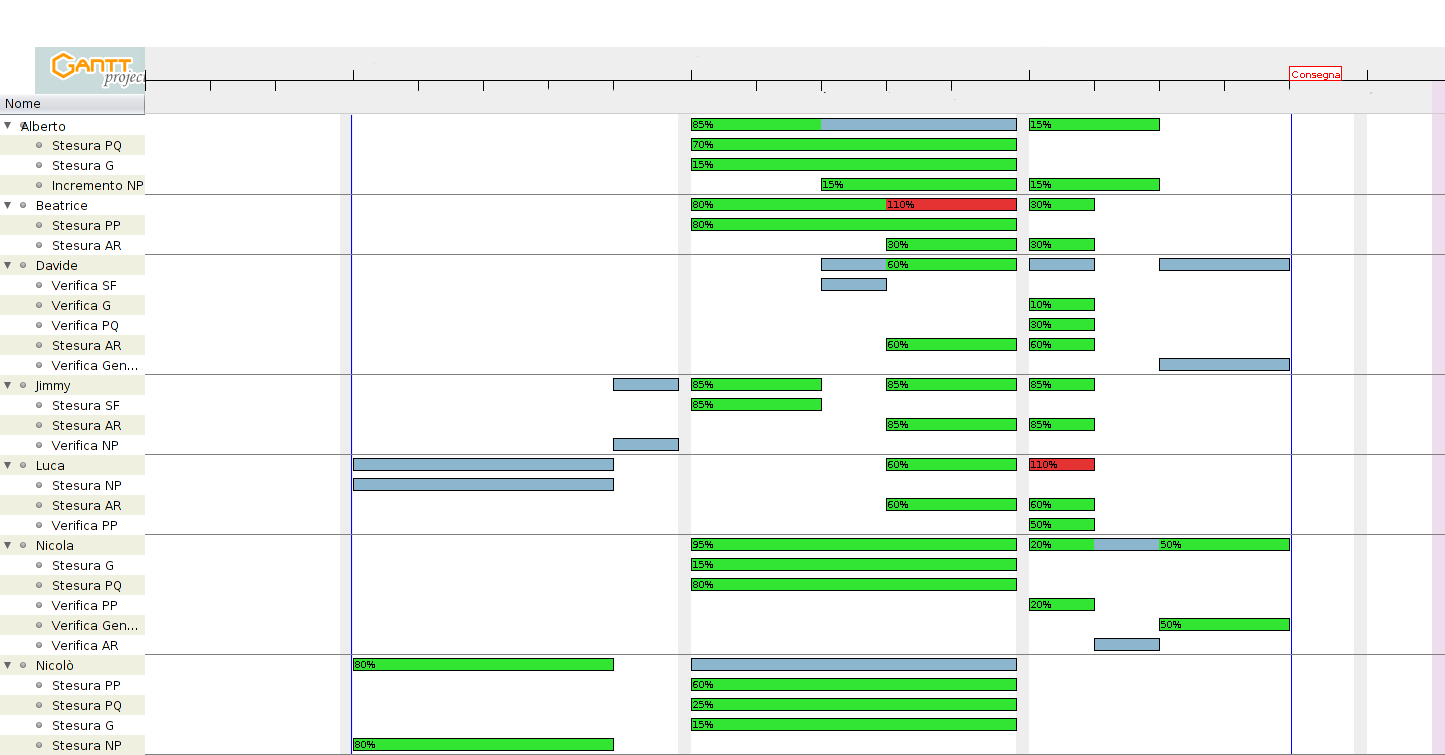
\includegraphics[width=\linewidth]{./content/Immagini/AnalisiR.png}
	\caption{Attività a Risorsa, Fase A}
\end{figure}
\end{landscape}
\pagebreak
\subsubsection{Prospetto economico}
\label{costoAnalisi}
Nella fase A, le ore ripartite tra i ruoli (sezione \ref{Analisi}) e i conseguenti costi sono evidenziati nella seguente tabella:
\begin{table}[!h]
\tableEco
Amministratore & 20 & 400\\
Responsabile & 18 & 540\\
Analista & 65 & 1.625\\
Verificatore & 41 & 902\\
Progettista & &\\
Programmatore & &\\
\cline{2-3} 
&144 & 3.467\\ \hline
\end{tabular}\caption{Costi a Ruolo, Fase A}
\end{center}
\end{table}
\\
I valori sono riassunti nel seguente grafico a torta che espone l'incidenza dei costi per ruolo
\begin{figure}[h]
	\centering
	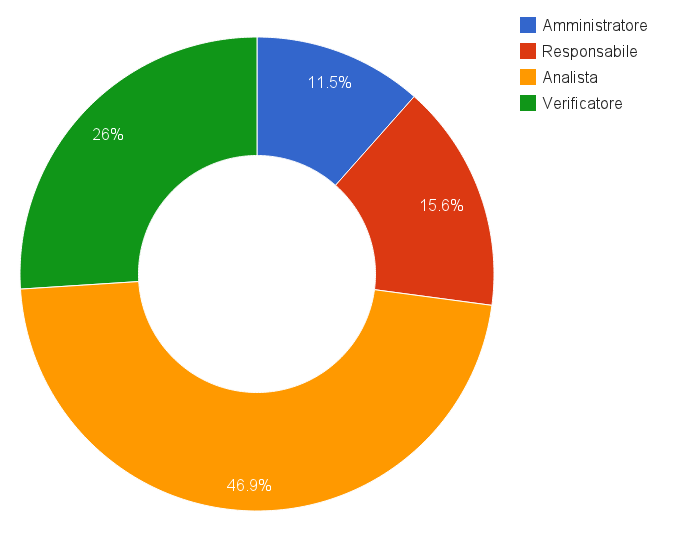
\includegraphics[width=0.9\linewidth]{./content/Immagini/prospetti/costiAn.png}
	\caption{Incidenza Costi a Ruolo, Fase A}
\end{figure}
\pagebreak
%%%%%%%%%%%%%%%%%%%%%%%%%%%%%%%%%%%%%%%%%%%%%%%%%%
% ANALISI INCREMENTALE
%%%%%%%%%%%%%%%%%%%%%%%%%%%%%%%%%%%%%%%%%%%%%%%%%%
\subsection{Fase B}
\label{AnalisiIncrementaleLav}
\subsubsection{Suddiviosione del lavoro}
\label{lavoroB}
Nella FB, ciascun componente dovrà rivestire i ruoli come illustrato nella tabella seguente:
\begin{table}[!h]
\tableResource
Adami Alberto & & & & 8 & & & 8\\
Bissacco Nicolò & & & 7 & & & & 7\\
Feltre Beatrice & & & & 8 & & & 8\\
Luisetto Luca & & 3 & & 6 & & & 9\\
Magnabosco Nicola & & & 9 & & & & 9\\
Martignago Jimmy & & & 8 & & & & 8\\
Scapin Davide & 7 & & 3 & & & & 10\\ \hline
\end{tabular} \caption{Ore a Componente per Ruolo, Fase B}
\end{center}
\end{table}
\\ I valori sono riassunti nel seguente grafico che visualizza le ore che un membro ha ricoperto in un determinato ruolo.
\begin{figure}[h]
	\centering
	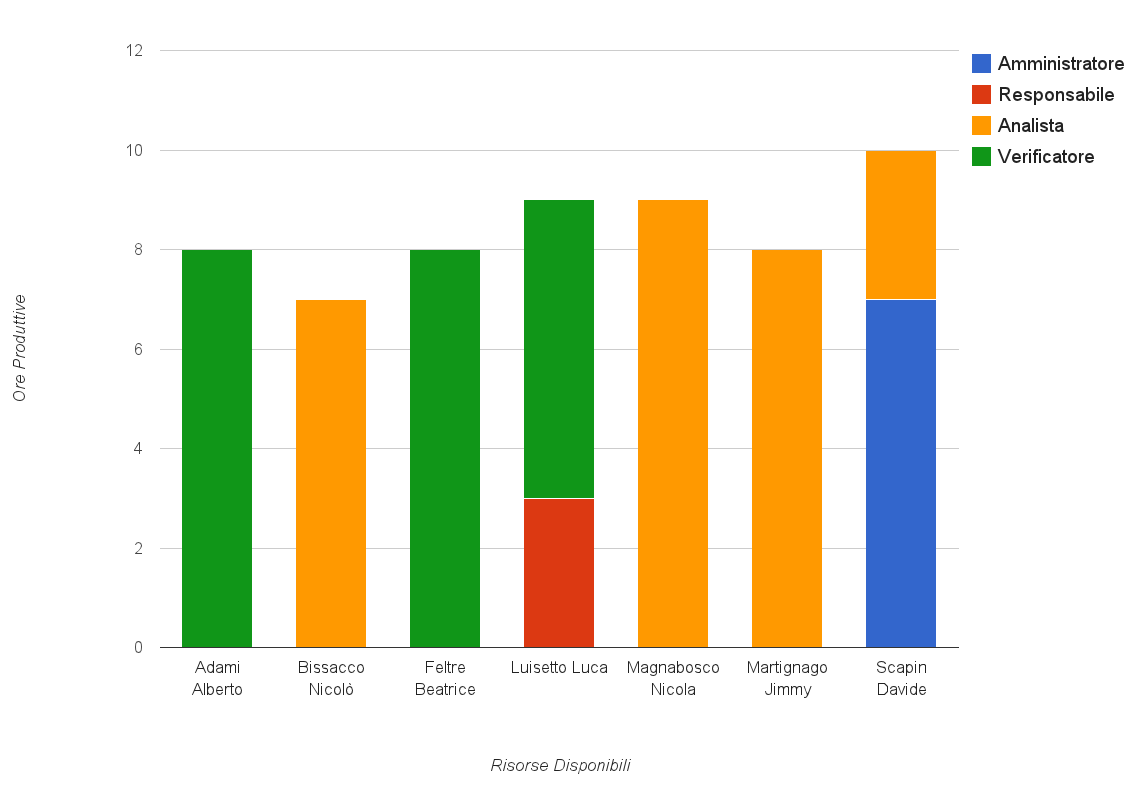
\includegraphics[width=\linewidth]{./content/Immagini/prospetti/risorseAnIn.png}
	\caption{Ore per Componente, Fase B}
\end{figure}

Il diagramma che segue rappresenta le attività effettive assegnate ad ogni risorsa e la percentuale di tempo dedicato ad essa, evidenziando in rosso, quelle risorse che si trovano sovraccaricate e in verde quelle invece che sono sottoccupate.
\begin{landscape}
\begin{figure}[h]
	\centering
	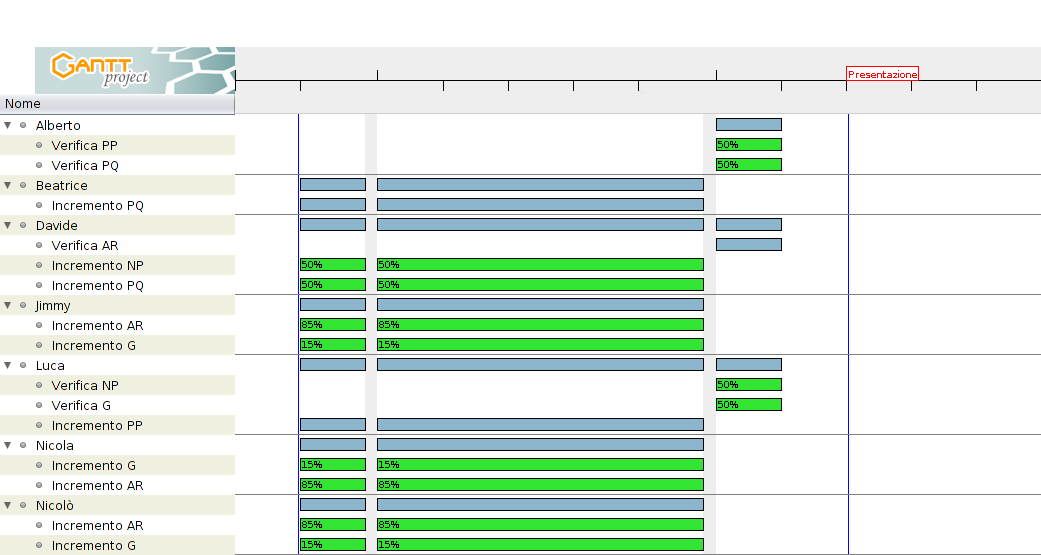
\includegraphics[width=\linewidth]{./content/Immagini/Analisi_incrementaleR.png}
	\caption{Attività a Risorsa, Fase B}
\end{figure}
\end{landscape}
\subsubsection{Prospetto economico}
\label{costoAnalisiIncrementale}
Nella fase B, le ore ripartite tra i ruoli (sezione \ref{AnalisiIncrementaleR}) e i conseguenti costi sono evidenziati nella seguente tabella:
\begin{table}[!h]
\tableEco
Amministratore & 7 & 140\\
Responsabile & 3 & 90\\
Analista & 27 & 675\\
Verificatore & 22 & 484\\
Progettista & &\\
Programmatore & &\\
\cline{2-3} 
&59 & 1.389\\ \hline
\end{tabular}\caption{Costi a Ruolo, Fase B}
\end{center}
\end{table}
I valori sono riassunti nel seguente grafico a torta che espone l'incidenza dei costi per ruolo
\begin{figure}[h]
	\centering
	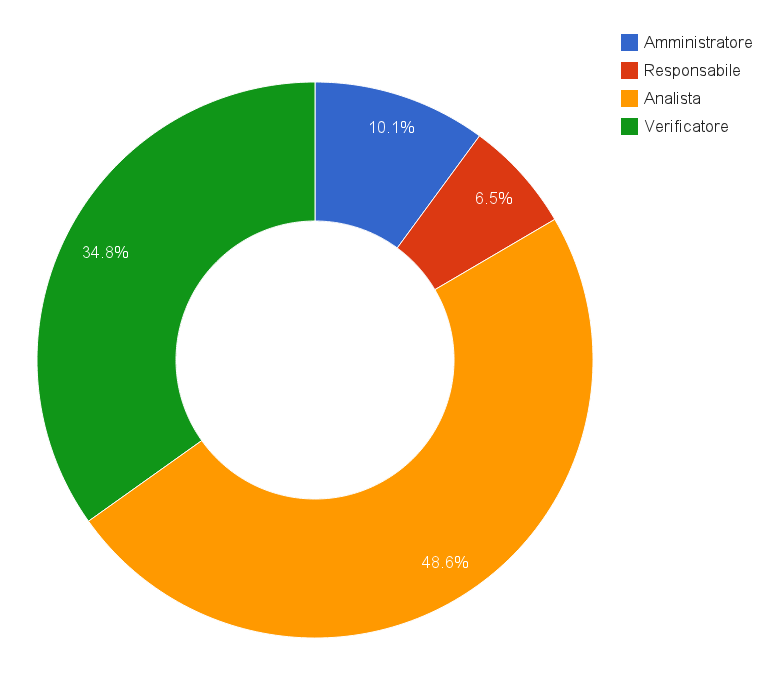
\includegraphics[width=0.9\linewidth]{./content/Immagini/prospetti/costiAnIn.png}
	\caption{Incidenza Costi a Ruolo, Fase B}
\end{figure}
\pagebreak
%%%%%%%%%%%%%%%%%%%%%%%%%%%%%%%%%%%%%%%%%%%%%%%%%%
% progettazione
%%%%%%%%%%%%%%%%%%%%%%%%%%%%%%%%%%%%%%%%%%%%%%%%%%
\subsection{Fase C}
\label{ProgettazioneArchitetturaleLav}
\subsubsection{Suddiviosione del lavoro}
\label{lavoroC}
Nella FC, ciascun componente dovrà rivestire i ruoli come illustrato nella tabella seguente:
\begin{table} [!h]
\tableResource
Adami Alberto & & 5& 10& & 9& & 24\\
Bissacco Nicolò & & & &20 & 6& & 26\\
Feltre Beatrice &4 & & & & 22& & 26\\
Luisetto Luca &4 & & &  & 23& & 27\\
Magnabosco Nicola & & 4& 9 & & 14& & 27\\
Martignago Jimmy & &2 & &18 & 6& & 26\\
Scapin Davide & & &  &8 &19 & & 27\\ \hline
\end{tabular} \caption{Ore a Componente per Ruolo, Fase C}
\end{center}
\end{table}
\\ I valori sono riassunti nel seguente grafico che visualizza le ore che un membro ha ricoperto in un determinato ruolo.
\begin{figure}[!h]
	\centering
	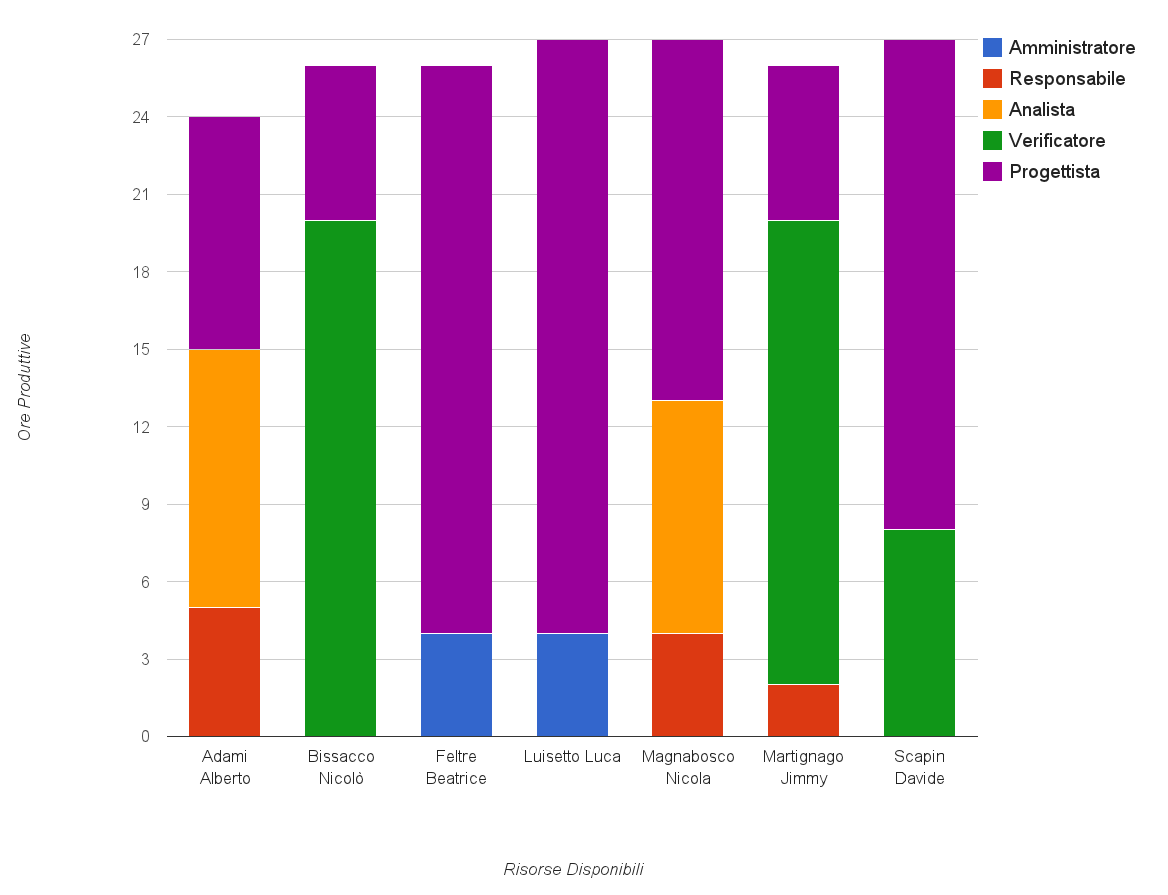
\includegraphics[width=1.05\linewidth]{./content/Immagini/prospetti/risorsePrAn.png}
	\caption{Ore per Componente, Fase C}
\end{figure}

Il diagramma che segue rappresenta le attività effettive assegnate ad ogni risorsa e la percentuale di tempo dedicato ad essa, evidenziando in rosso, quelle risorse che si trovano sovraccaricate e in verde quelle invece che sono sottoccupate.
\begin{landscape}
\begin{figure}[!h]
	\centering
	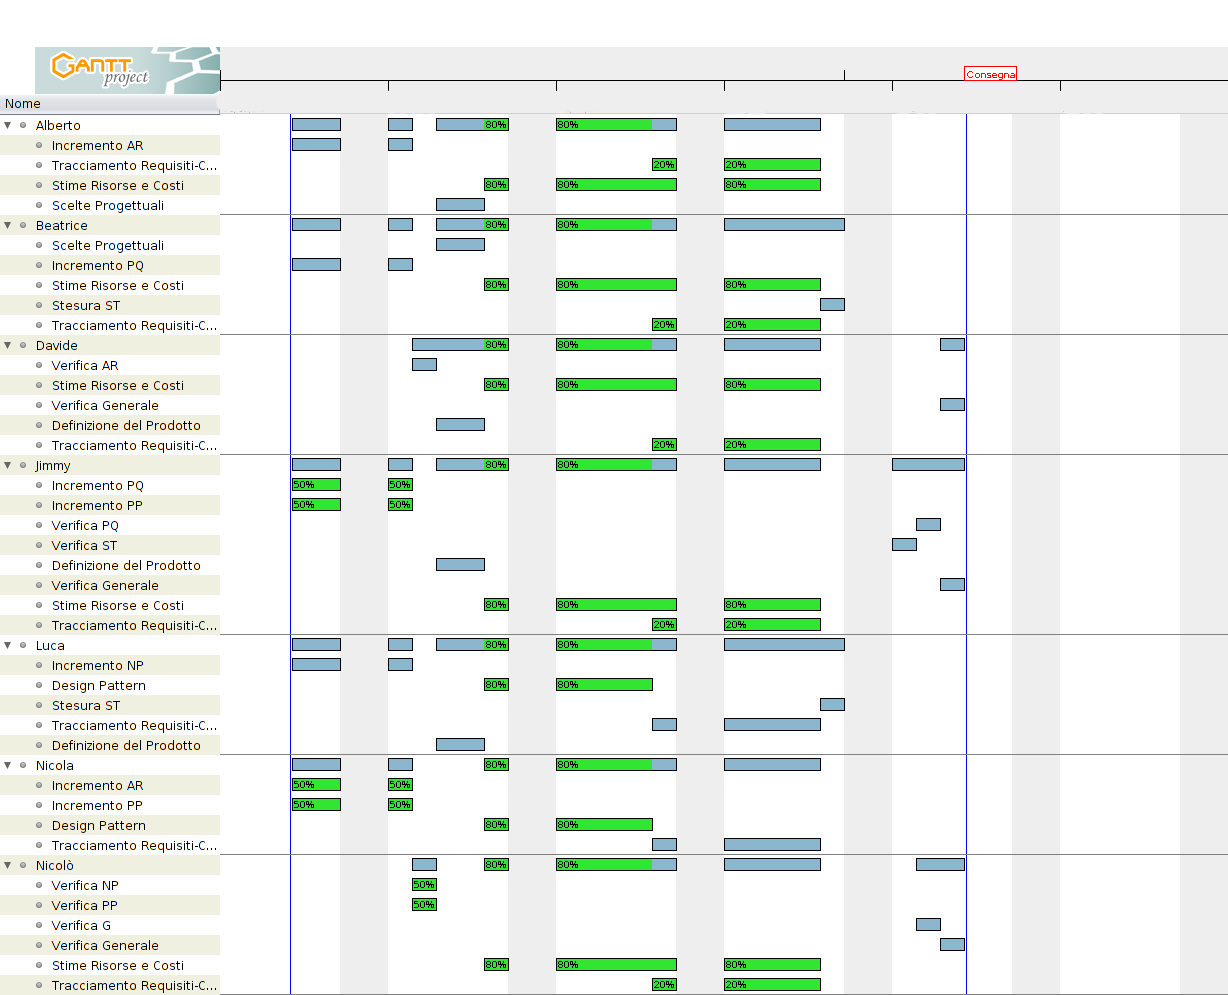
\includegraphics[width=0.85\linewidth]{./content/Immagini/Progettazione_architetturaleR.png}
	\caption{Attività a Risorsa, Progettazione Architetturale}
\end{figure}
\end{landscape}
\pagebreak
\subsubsection{Prospetto economico}
\label{costoProgettazioneArchitetturale}
Nella fase C, le ore ripartite tra i ruoli (sezione \ref{ProgettazioneArchitetturaleR}) e i conseguenti costi sono evidenziati nella seguente tabella:
\begin{table}[!h]
\tableEco
Amministratore & 8 & 160\\
Responsabile & 11 & 330\\
Analista & 19 & 475\\
Verificatore & 46 & 1.012\\
Progettista & 99&1.485\\
Programmatore & &\\
\cline{2-3} 
&183 & 3.462\\ \hline
\end{tabular}\caption{Costi a Ruolo, Fase C}
\end{center}
\end{table}

I valori sono riassunti nel seguente grafico a torta che espone l'incidenza dei costi per ruolo
\begin{figure}[h]
	\centering
	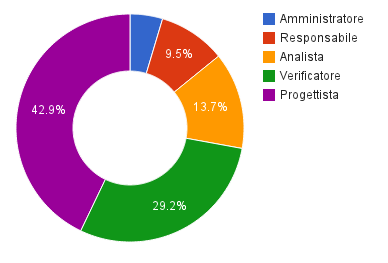
\includegraphics[width=0.8\linewidth]{./content/Immagini/prospetti/costiPrAr.png}
	\caption{Incidenza Costi a Ruolo, Fase C}
\end{figure}
\pagebreak
%%%%%%%%%%%%%%%%%%%%%%%%%%%%%%%%%%%%%%%%%%%%%%%%%%
% codifica
%%%%%%%%%%%%%%%%%%%%%%%%%%%%%%%%%%%%%%%%%%%%%%%%%%
\subsection{Fase D}
\label{ProgettazioneDettaglioLav}
\subsubsection{Suddiviosione del lavoro}
\label{lavoroD}
Nella FD, ciascun componente dovrà rivestire i ruoli come illustrato nella tabella seguente:
\begin{table}[!h]
\tableResource
Adami Alberto & & & & 28 &23 & & 51\\
Bissacco Nicolò & & & &17 &25 &10 & 52\\
Feltre Beatrice & & & & 30 &22 & & 52\\
Luisetto Luca & &  & & 25& & 26& 51\\
Magnabosco Nicola & 9& & & &4 &40 & 53\\
Martignago Jimmy & & & 3 & &31 &14 & 48\\
Scapin Davide &  &11 & &11 & & 28& 50\\ \hline
\end{tabular}
\caption{Ore a Componente per Ruolo, Fase D}
\end{center}
\end{table}
\\ I valori sono riassunti nel seguente grafico che visualizza le ore che un membro ha ricoperto in un determinato ruolo.
\begin{figure}[!h]
	\centering
	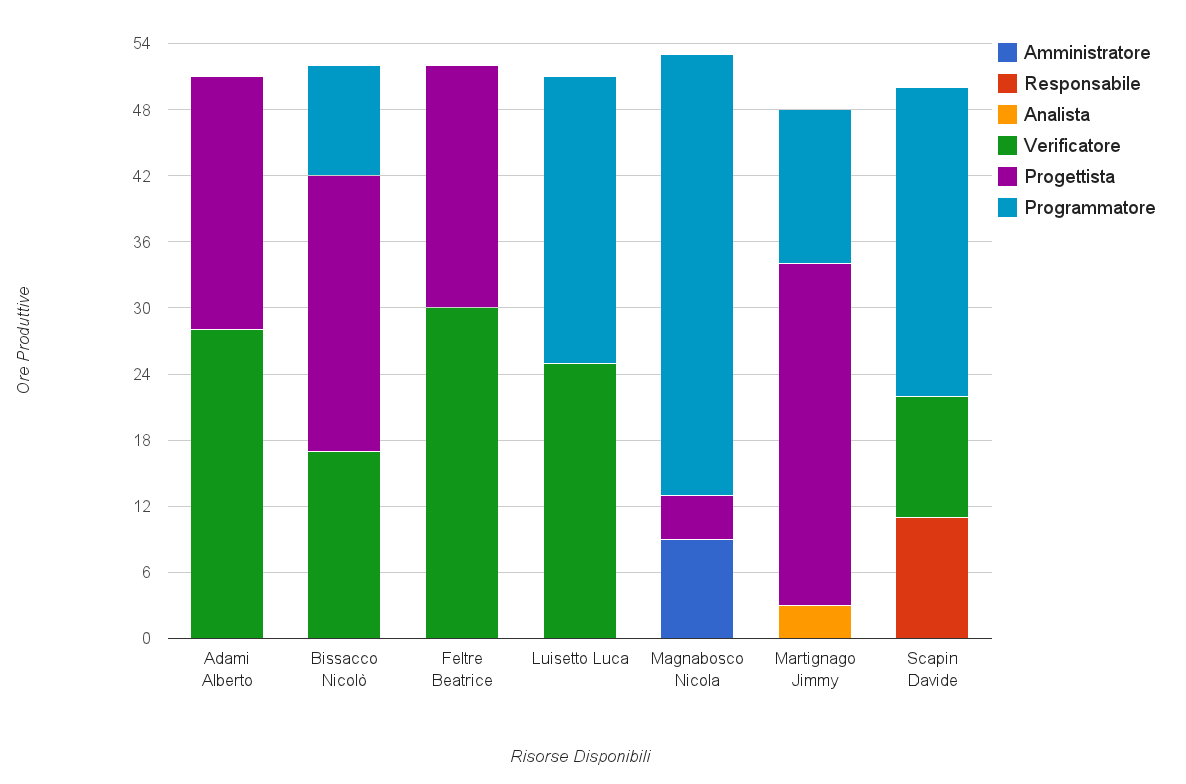
\includegraphics[width=\linewidth]{./content/Immagini/prospetti/risorsePrDe.png}
	\caption{Ore per Componente, Fase D}
\end{figure}

Il diagramma che segue rappresenta le attività effettive assegnate ad ogni risorsa e la percentuale di tempo dedicato ad essa, evidenziando in rosso, quelle risorse che si trovano sovraccaricate e in verde quelle invece che sono sottoccupate.
\begin{landscape}
\begin{figure}[!h]
	\centering
	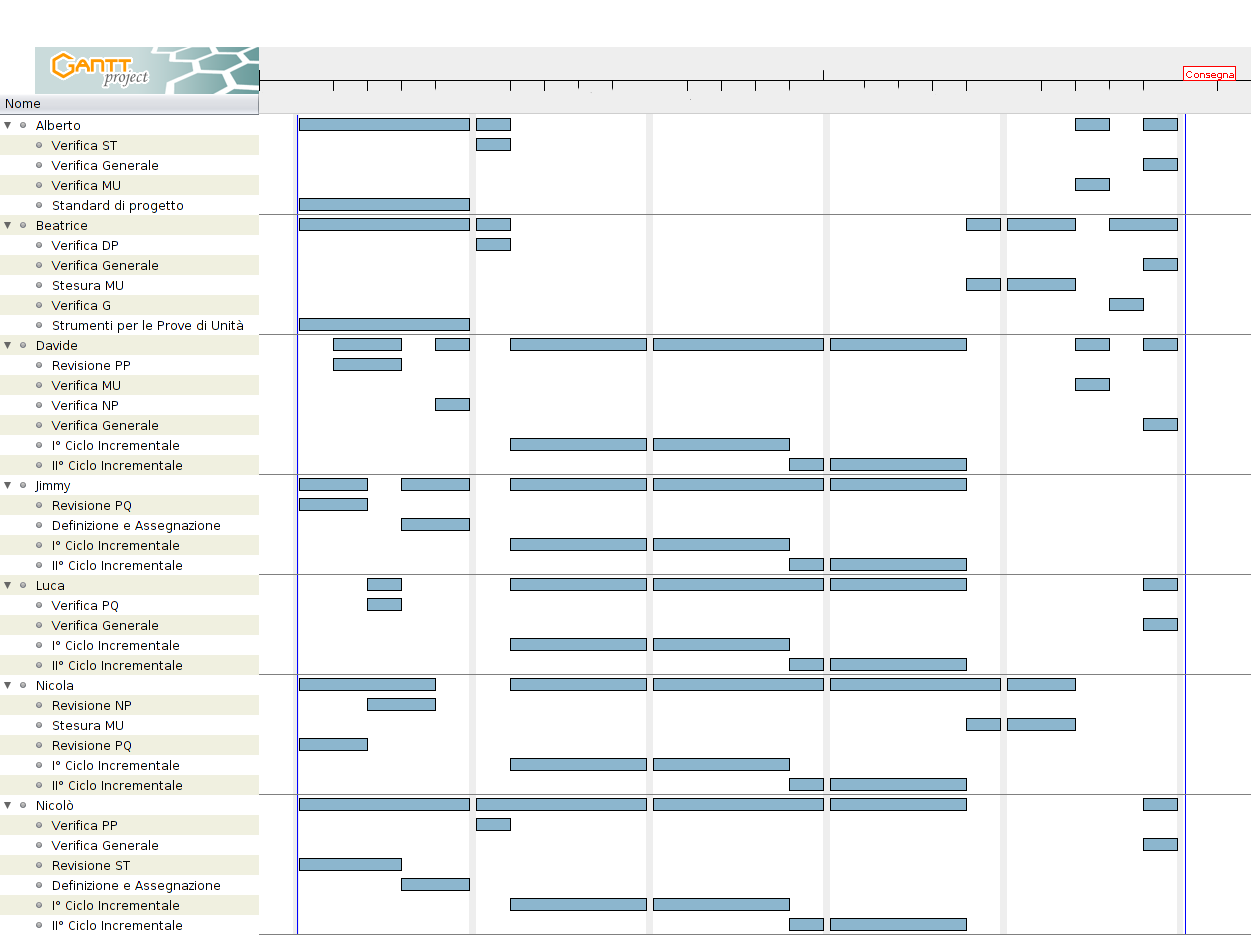
\includegraphics[width=0.85\linewidth]{./content/Immagini/Progettazione_dettaglio_codificaR.png}
	\caption{Attività a Risorsa, Fase D}
\end{figure}
\end{landscape}
\pagebreak
\subsubsection{Prospetto economico}
\label{costoProgettazioneDettaglio}
Nella fase D, le ore ripartite tra i ruoli (sezione \ref{ProgettazioneDettaglioR}) e i conseguenti costi sono evidenziati nella seguente tabella:
\begin{table}[!h]
\tableEco
Amministratore & 9 & 180\\
Responsabile & 11 & 330\\
Analista & 3 & 75\\
Verificatore & 111 & 2.442\\
Progettista &105 &1.575\\
Programmatore &188 &1.770\\
\cline{2-3} 
&357 & 6.372\\ \hline
\end{tabular}\caption{Costi a Ruolo, Fase D}
\end{center}
\end{table}

I valori sono riassunti nel seguente grafico a torta che espone l'incidenza dei costi per ruolo
\begin{figure}[h]
	\centering
	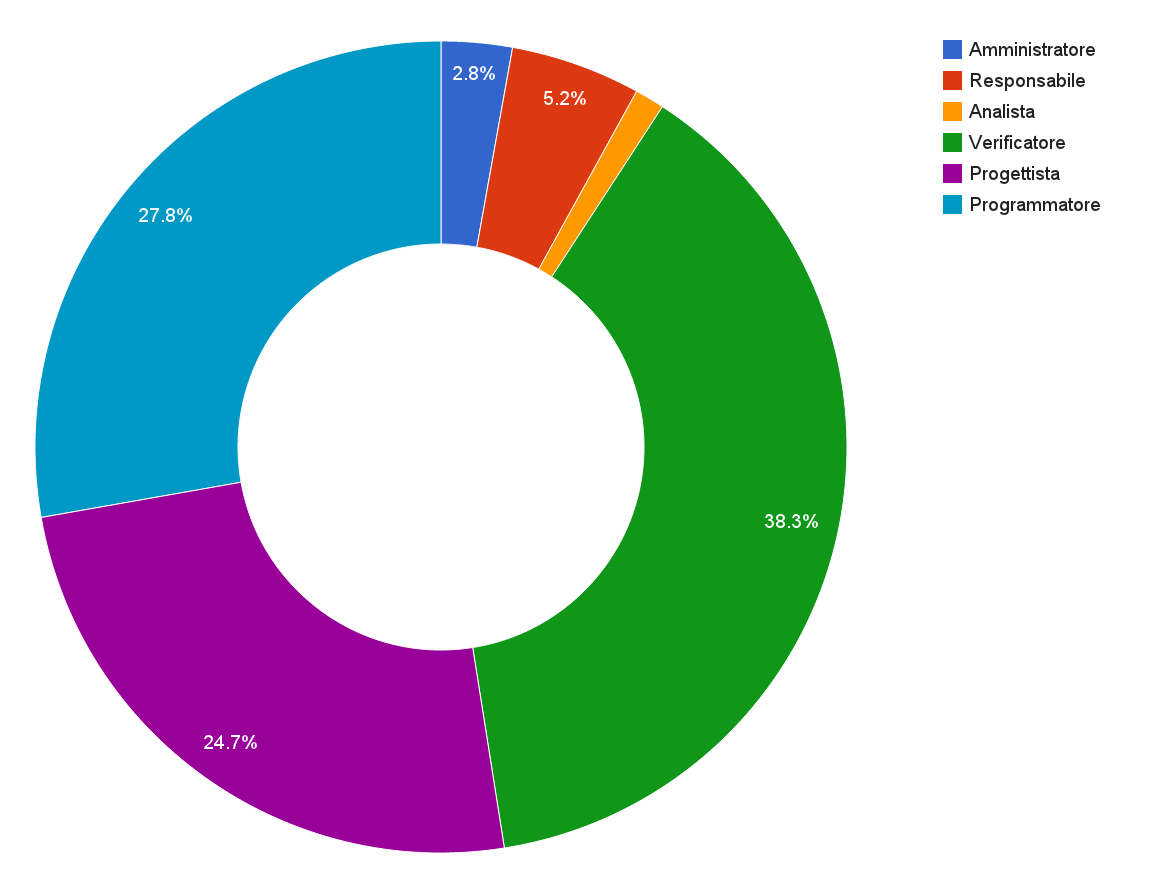
\includegraphics[width=0.8\linewidth]{./content/Immagini/prospetti/costiPrDe.png}
	\caption{Incidenza Costi a Ruolo, Fase D}
\end{figure}
\pagebreak
%%%%%%%%%%%%%%%%%%%%%%%%%%%%%%%%%%%%%%%%%%%%%%%%%%
% verifica e validazione
%%%%%%%%%%%%%%%%%%%%%%%%%%%%%%%%%%%%%%%%%%%%%%%%%%
\subsection{Fase E}
\label{VerificaValidazioneLav}
\subsubsection{Suddiviosione del lavoro}
\label{lavoroE}
Nella FE, ciascun componente dovrà rivestire i ruoli come illustrato nella tabella seguente:
\begin{table} [!h]
\tableResource
Adami Alberto & & & & 10& & 7& 17\\
Bissacco Nicolò & & & &15 & & & 15\\
Feltre Beatrice & 7& & &2 & &7 & 16\\
Luisetto Luca & &7 & & & 8& & 15\\
Magnabosco Nicola & & & &9 & 5& & 14\\
Martignago Jimmy &2 & & &17 & & &19\\
Scapin Davide & & & & 8&7& & 15\\ \hline
\end{tabular} \caption{Ore a Componente per Ruolo, Fase E}
\end{center}
\end{table}
\\ I valori sono riassunti nel seguente grafico che visualizza le ore che un membro ha ricoperto in un determinato ruolo.
\begin{figure}[!h]
	\centering
	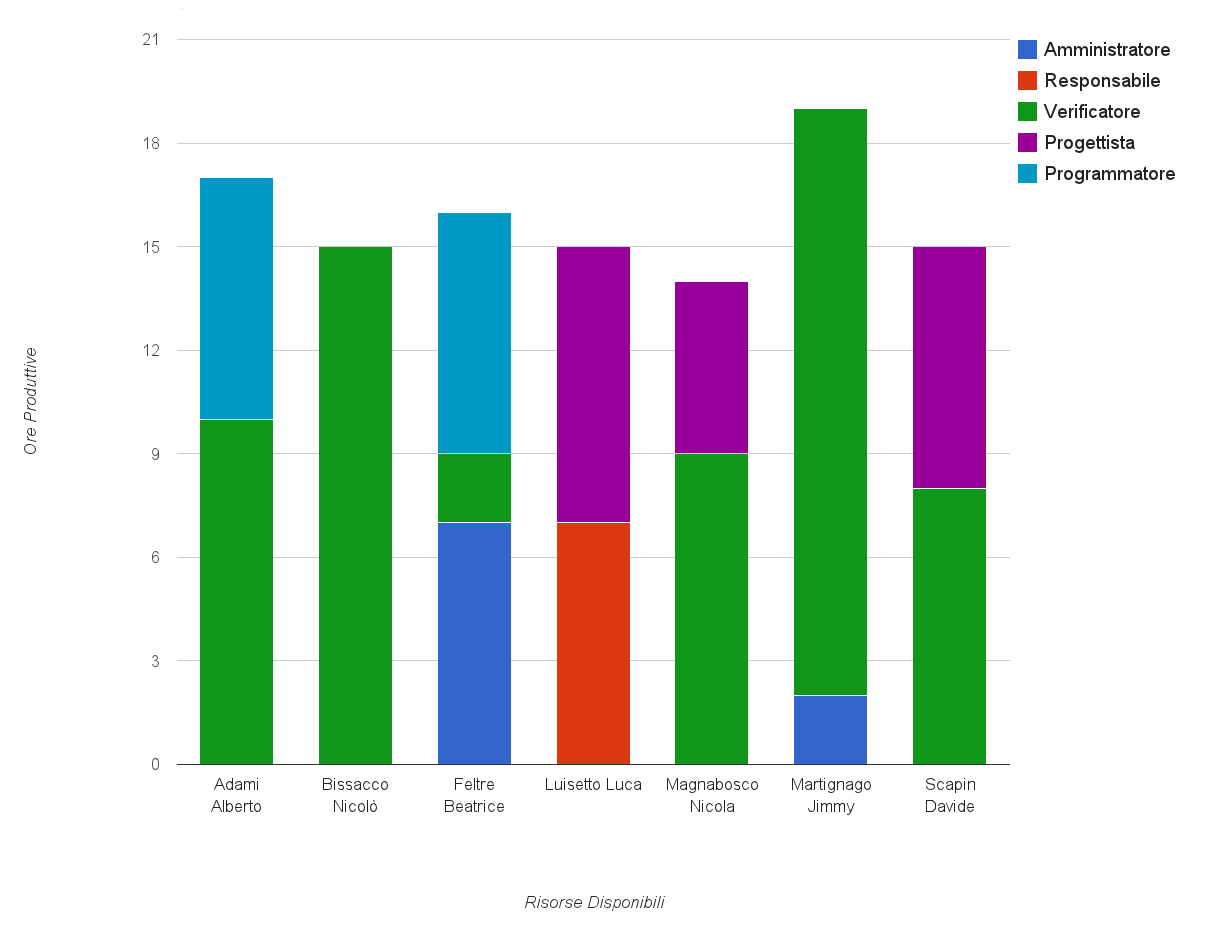
\includegraphics[width=0.9\linewidth]{./content/Immagini/prospetti/risorseVV.png}
	\caption{Ore per Componente, Verifica e Validazione}
\end{figure}

Il diagramma che segue rappresenta le attività effettive assegnate ad ogni risorsa e la percentuale di tempo dedicato ad essa, evidenziando in rosso, quelle risorse che si trovano sovraccaricate e in verde quelle invece che sono sottoccupate.
\begin{landscape}
\begin{figure}[!h]
	\centering
	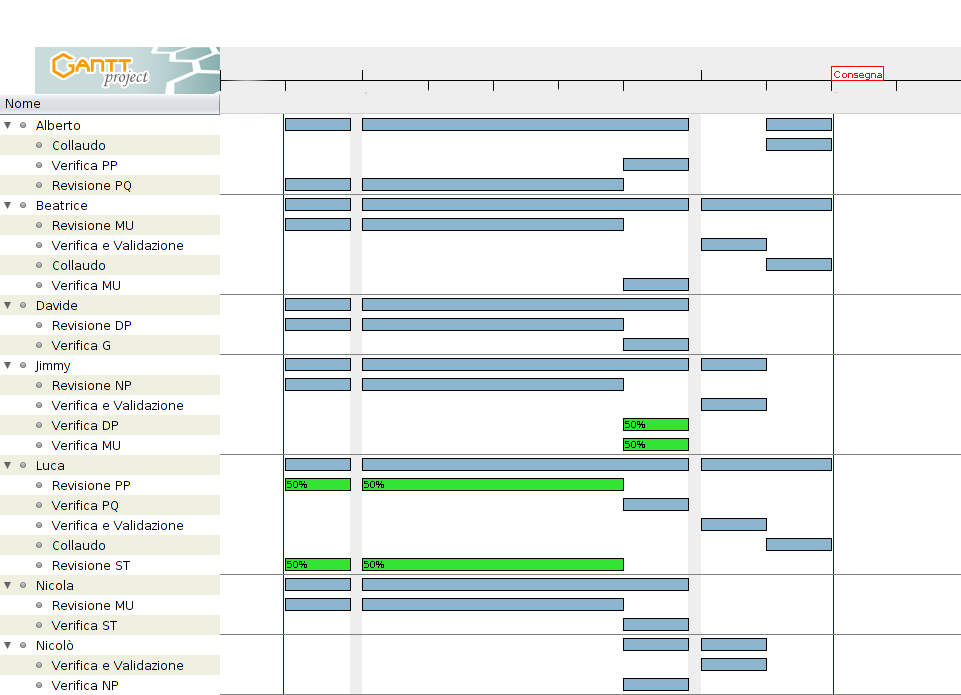
\includegraphics[width=0.85\linewidth]{./content/Immagini/Verifica_validazioneR.png}
	\caption{Attività a Risorsa, Fase E}
\end{figure}
\end{landscape}
\pagebreak
\subsubsection{Prospetto economico}
\label{costoVerificaValidazione}
Nella fase E, le ore ripartite tra i ruoli (sezione \ref{VerificaValidazioneR}) e i conseguenti costi sono evidenziati nella seguente tabella:
\begin{table}[!h]
\tableEco
Amministratore & 9 & 180\\
Responsabile & 7 & 210\\
Analista &  & \\
Verificatore & 61 & 1.342\\
Progettista &20 &300\\
Programmatore &14 &210\\
\cline{2-3} 
&111 & 2.242\\ \hline
\end{tabular}\caption{Costi a Ruolo, Fase E}
\end{center}
\end{table}

I valori sono riassunti nel seguente grafico a torta che espone l'incidenza dei costi per ruolo
\begin{figure}[!h]
	\centering
	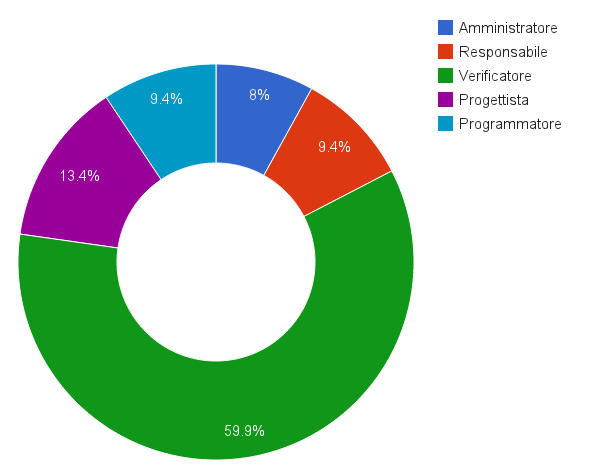
\includegraphics[width=0.9\linewidth]{./content/Immagini/prospetti/costiVV.png}
	\caption{Incidenza Costi a Ruolo, Fase E}
\end{figure}
\pagebreak

%%%%%%%%%% totali %%%%%%%%%%%
\subsection{Totali}
\label{TotaliLav}
\subsubsection{Totale ore}
\label{totore}
La tabella seguente illustra le ore totali che ogni componente dedicherà per il progetto, mettendo in evidenza anche quelle che verranno poi rendicontate.
\begin{table}[!h]
\centering
	\begin{tabular}{|l|l|c|c|c|c|c|c|c|}
	\cline{1-9}{\multirow{2}{*}{Nominativi}}& &\multicolumn{6}{c|}{Ore a Ruolo} & \multirow{2}{*}{Totali}\\
	&& Ad & Re & An & Ve & Pj & Pr& \\
	\hline
	\hline
	%Adami Alberto
	\multicolumn{1}{|l|}{\multirow{2}{*}{Adami Alberto}} & \multicolumn{1}{|l|}{Totali} & 10 &5&17&49&32&7&120\\
	\cline{2-9}
	&\multicolumn{1}{|l|}{Rendicontati} &&5&10&46&32&7&100\\
	\hline
	\hline
	% Bissacco Nicolò
		\multicolumn{1}{|l|}{\multirow{2}{*}{Bissacco Nicolò}} & \multicolumn{1}{|l|}{Totali} & 10 &4&14&52&31&10&121\\
	\cline{2-9}
	&\multicolumn{1}{|l|}{Rendicontati} &&&7&52&31&10&100\\
	\hline
	\hline
	%Feltre Beatrice
		\multicolumn{1}{|l|}{\multirow{2}{*}{Feltre Beatrice}} & \multicolumn{1}{|l|}{Totali} & 11 &8&12&40&44&7&122\\
	\cline{2-9}
	&\multicolumn{1}{|l|}{Rendicontati} &11&&&40&44&7&102\\
	\hline
	\hline
	%Luisetto Luca
			\multicolumn{1}{|l|}{\multirow{2}{*}{Luisetto Luca}} & \multicolumn{1}{|l|}{Totali} & 4 &10&13&39&31&26&123\\
	\cline{2-9}
	&\multicolumn{1}{|l|}{Rendicontati} &4&10&&31&31&26&102\\
	\hline
	\hline
	%Magnabosco Nicola
			\multicolumn{1}{|l|}{\multirow{2}{*}{Magnabosco Nicola}} & \multicolumn{1}{|l|}{Totali} & 9 &10&18&24&23&40&124\\
	\cline{2-9}
	&\multicolumn{1}{|l|}{Rendicontati} &9&4&18&9&23&40&103\\
	\hline
	\hline
	%Martignago Jimmy
			\multicolumn{1}{|l|}{\multirow{2}{*}{Martignago Jimmy}} & \multicolumn{1}{|l|}{Totali} & 2 &2&26&41&37&14&122\\
	\cline{2-9}
	&\multicolumn{1}{|l|}{Rendicontati} &2&2&11&35&37&14&101\\
	\hline
	\hline
	%Scapin Davide
			\multicolumn{1}{|l|}{\multirow{2}{*}{Scapin Davide}} & \multicolumn{1}{|l|}{Totali} & 7 &11&14&36&26&28&122\\
	\cline{2-9}
	&\multicolumn{1}{|l|}{Rendicontati} &7&11&3&27&26&28&102\\
	\cline{1-9}
	\cline{1-9}
	\end{tabular}
	\caption{Ore a Componente per Ruolo, Totali e Rendicontate}
	\label{componenteOre}
\end{table}
\pagebreak

I valori sono riassunti nei seguenti grafici che visualizzano le ore che un membro ha ricoperto in un determinato ruolo, nel complesso e rendicontate.
\begin{figure}[!h]
	\centering
	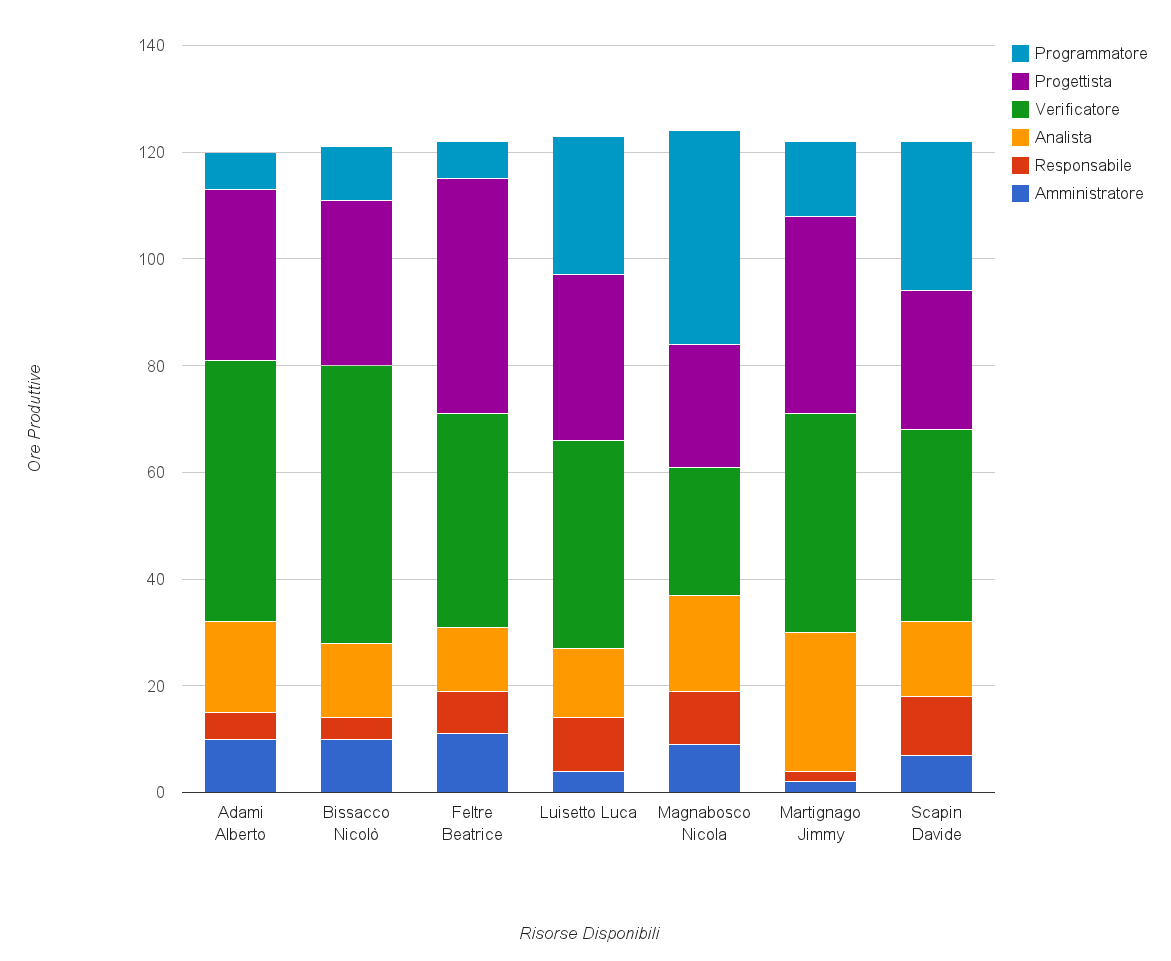
\includegraphics[width=\linewidth]{./content/Immagini/prospetti/costiRisTot.png}
	\caption{Ore per Componente, Totali}
\end{figure}
\begin{figure}[!h]
	\centering
	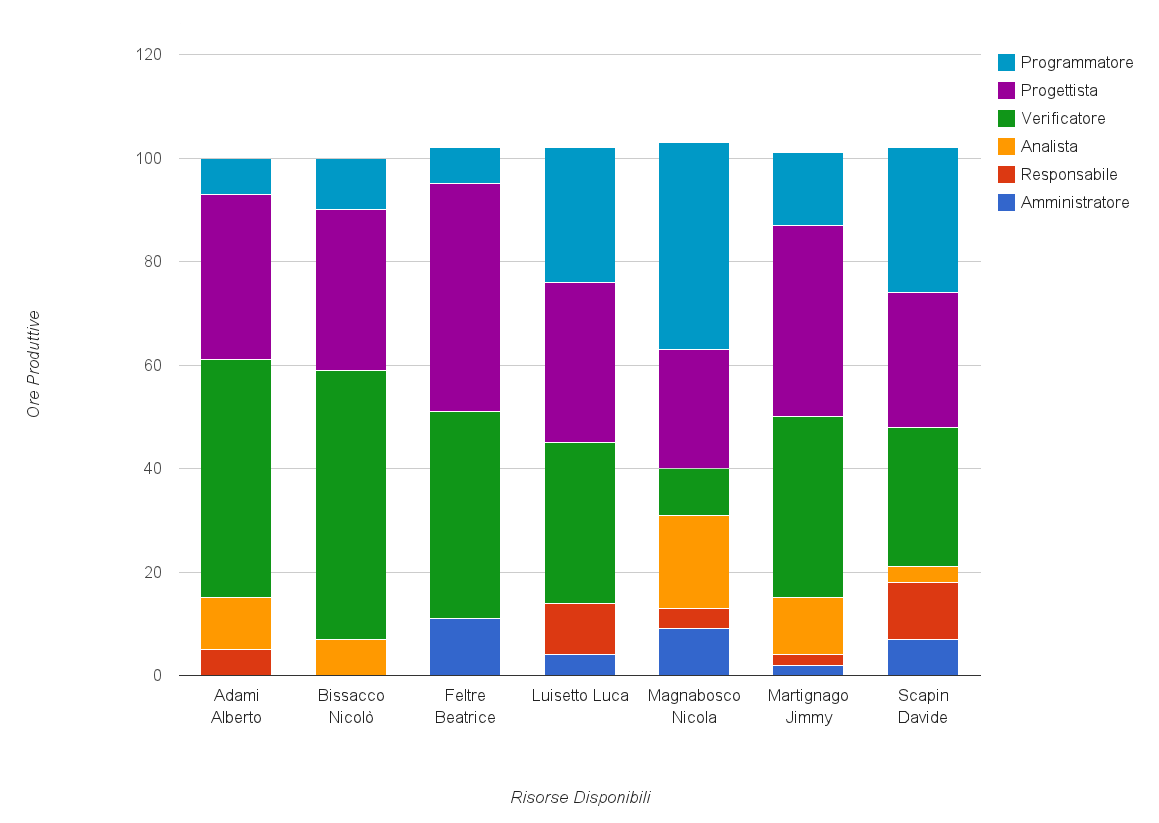
\includegraphics[width=\linewidth]{./content/Immagini/prospetti/oreRisorseRem.png}
	\caption{Ore per Componente, Rendicontate}
\end{figure}

\subsubsection{Totale costi}
La tabella seguente ha il compito di illustrare le ore totali e rendicontate previste per la realizzazione di \project{} suddivise per ruoli
\begin{table}[!h]
	\centering
	\begin{tabular}{|l|l|c|c|}
		\hline
			Ruolo& & Ore & Costo\\ \hline
			\multicolumn{1}{|l|}{\multirow{2}{*}{Amministratore}} & \multicolumn{1}{|l|}{Totale} & 53 & 1.060 \\
			\cline{2-4}
			&\multicolumn{1}{|l|}{Rendicontato} &33&660\\
		\hline
		\hline
			%responsabile
			\multicolumn{1}{|l|}{\multirow{2}{*}{Responsabile}} & \multicolumn{1}{|l|}{Totale} & 50 & 1.500\\
			\cline{2-4}
			&\multicolumn{1}{|l|}{Rendicontato} &32&960\\
		\hline
		\hline
			%Analista
			\multicolumn{1}{|l|}{\multirow{2}{*}{Analista}} & \multicolumn{1}{|l|}{Totale} & 114 &2.850\\
			\cline{2-4}
			&\multicolumn{1}{|l|}{Rendicontato} &49&1.225\\
		\hline
		\hline
			%Verificatore
			\multicolumn{1}{|l|}{\multirow{2}{*}{Verificatore}} & \multicolumn{1}{|l|}{Totale} & 281 &6.182\\
			\cline{2-4}
			&\multicolumn{1}{|l|}{Rendicontato} &240 & 5.280\\
		\hline
		\hline
			%progettista
			\multicolumn{1}{|l|}{\multirow{2}{*}{Progettista}} & \multicolumn{1}{|l|}{Totale} & 281 &6.182\\
			\cline{2-4}
			&\multicolumn{1}{|l|}{Rendicontato} &240 & 5.280\\
		\hline
		\hline
			%Programmatore
			\multicolumn{1}{|l|}{\multirow{2}{*}{Programmatore}} & \multicolumn{1}{|l|}{Totale} & 281 &6.182\\
			\cline{2-4}
			&\multicolumn{1}{|l|}{Rendicontato} &240 & 5.280\\
		\hline
		\hline
			%Totali
			\multicolumn{1}{|l|}{\multirow{2}{*}{}} & \multicolumn{1}{|l|}{Totale} &854  &16.932\\
			\cline{2-4}
			&\multicolumn{1}{|l|}{Rendicontato} & \textbf{710} & \textbf{13.465}\\
		\hline
		\hline
	\end{tabular}
	\caption{Prospetto Economico Preventivato}
	\label{prosp}
\end{table}
\\	
\\
\\
I valori sono riassunti nei seguenti grafici a torta che espongono l'incidenza dei costi per ruolo totali l'uno e l'incidenza dei costi rendicontati l'altro suddivisi per ruolo.
\begin{figure}[!h]
	\centering
	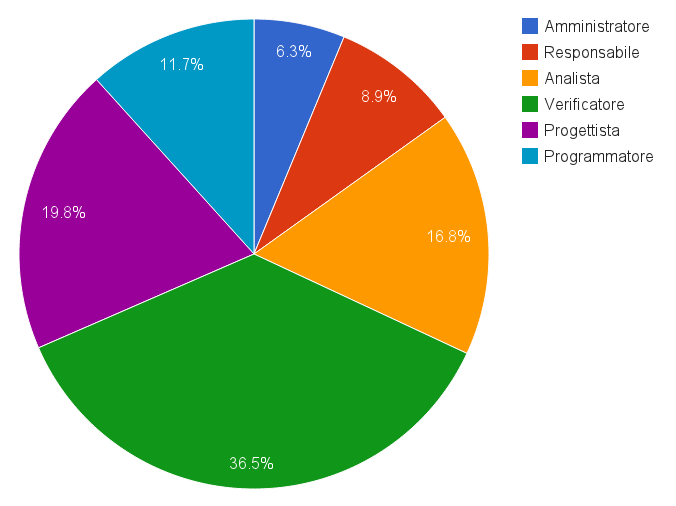
\includegraphics[width=0.9\linewidth]{./content/Immagini/prospetti/totruoloinvestim.png}
	\caption{Incidenza Costi a Ruolo, Totali}
\end{figure}
\pagebreak
\begin{figure}[!h]
	\centering
	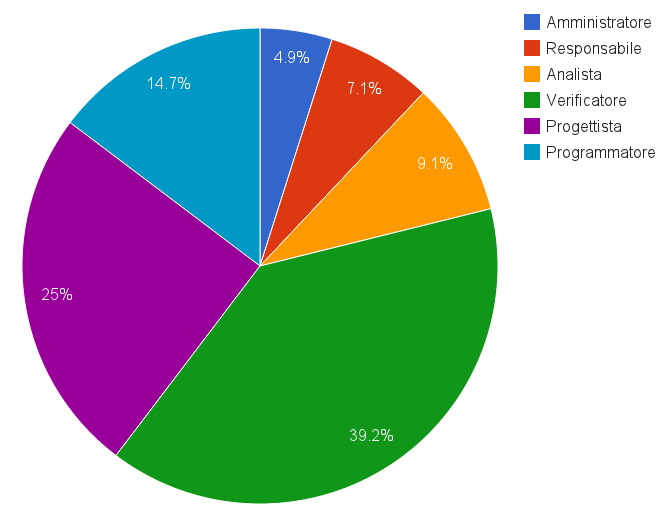
\includegraphics[width=0.9\linewidth]{./content/Immagini/prospetti/totaruoloremunerabili.png}
	\caption{Incidenza Costi a Ruolo, Rendicontati}
\end{figure}
\\
\\
\\
\subsection{Conclusioni}
\label{costiConclusioni}
Il costo totale per realizzare \project{} evidenziato in tabella \ref{prosp} e imputabile al proponente, è di \textbf{13.465 euro}; richiede 710 ore di sviluppo ovvero un totale di ore che va dalle 100 alle 103 a componente, come illustrato precedentemente nella tabella \ref{componenteOre}.

